Då $\bm{b}\times \bm{c}$ ger normalen, vilket är ortogonal till planet $\bm{bc}$ spänner. 
Detta leder till att vi får $\bm{a}\times \bm{n}$ som sedan är ortogonal mot normalen, dvs parallell med planet.
Eftersom den är parallell med planet, innebär det att normalens normal vektor kan representeras av någon linjär kombination av $\bm{b}$ och $\bm{c}$,
dvs $\lambda\bm{b} + \mu\bm{c}$.
\begin{center}
    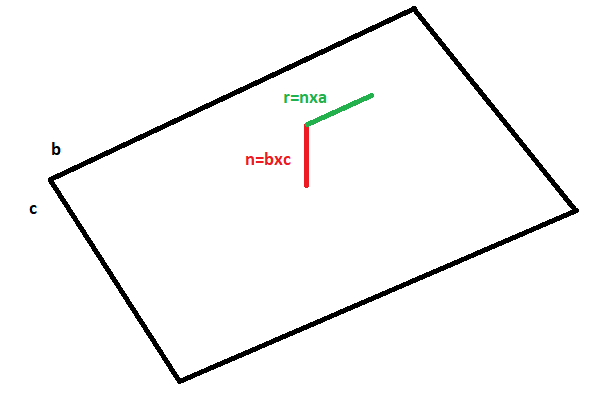
\includegraphics[scale=0.4]{imgs/bild2.png}
\end{center}